\pagebreak
\chapter{Visualizierung}
\label{chap:visualisierung}
\thispagestyle{empty}

\noindent Um die Visualisierung zu verbessern und nicht nur einzelne Punkte zu rendern haben wir uns für die erstellung eines Drahtgittermodells entschieden, welches aus unseren Datenstrukturen erstellt werden soll. Nach kurzer Recherche kamen wir somit auf Marching Cubes und in diesem Kapitel wird allgemein einmal der Algorithmus vorgestellt und speziell auf unsere Implementierung eingegangen.

\section{Marching Cubes}
\subsection{Allgemeine Beschreibung des Algorithmus}

\begin{center}
\emph{{\small Tobias Graf}}
\end{center}

\bigskip

\noindent Der Marching Cubes Algorithmus ziehlt darauf ab eine sogenannte Voxel - Datenmenge, ein Wurfelförmiges dreidimensionales Gitter aus Datenpunkten, in eine flächendeckende polygonale Oberfläche umzuwandeln und wird meistens für Medizische Anwendungen benutz. Da Computertomografen im allgemeinen bereits Voxel-Datenmengen liefern und für die Visualisierung der Ergebnisse Drahtgittermodelle benötigt werden, ist dies der größte Anwendungsbereich. 
\medskip
\noindent Hinweis: \textit{Für die allgemeine Erklärung wird nicht weiter auf die Erstellung von Voxel-Datenmengen eingegangen, im spezifischen Teil wird erläutert wie sie in unserem Projekt erstellt wird. }
\medskip
\noindent Zuerst wird das Datenmodell in einzelne Würfel unterteilt deren Eckpunkte die Voxel sind die die Dichte der Oberfläche an dem betreffendem Eckpunkt des Würfels darstellen. Abhängig davon ob eine gewisse Dichte erreicht wird muss in dem Würfel ein Drahtgittermodell erstellt werden welches die belegten Voxel verdeckt. Dazu werden an den Kanten des Würfels Vertices angelegt welche nach einem bestimmten Schema miteinander verknüpft werden. 
\begin{align*}
\noindent
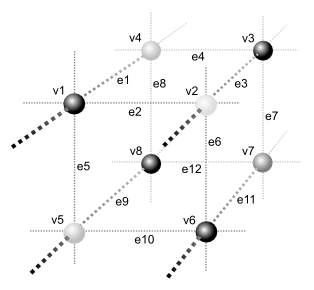
\includegraphics[scale=0.9]{images/Marching_Cubes_Kubus}
\end{align*}
\medskip 
\noindent Da sich pro Würfel acht Vertices und zwei Zustände (Innen und Aussen) ergeben sich $2^8 = 256$ Konfigurationen wie das Drahtgittermodell aufgebaut sein muss. Da jedoch die Triangulation der $256$ Konfigurationen ziemlich Fehleranfällig ist kann durch zwei Symmetrien eines Würfels das Problem auf $14$ Fälle (nach \cite{MC}) bzw. $17$ Fälle (nach \cite{MCADD}) reduziert werden. Zum einen ist die Topologie der triangulierten Oberfläche unverändert wenn sie nach Innen oder Aussen zeigt und Fälle mit $0$ bis $4$ Vertices für die Darstellung interessant sind reduziert sich das Konfigurationsspektrum bereits auf $128$. Als zweites kommt die Symmetrie der Rotation hinzu wodurch die $14$ Vorlagen ausreichen um die meisten Fälle abzudecken. 
\begin{align*}
\noindent
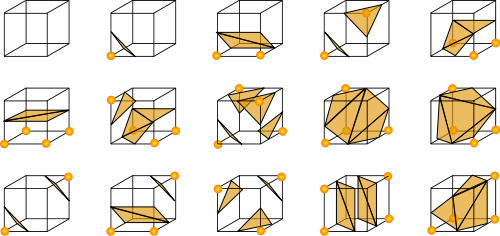
\includegraphics[scale=0.9]{images/MarchingCubesConfig}
\end{align*}
\medskip 
\noindent Die einfachste Konfiguration $0$ tritt auf wenn alle Voxel - Werte über (oder unter entsprechend Symmetrie eins) dem Schwellwert für die Darstellung liegen und generiert keine Dreiecke des Drahtgittermodells. Die nächste Vorlage $1$ tritt auf wenn lediglich ein Voxel - Wert die Bedingung erfüllt und erstellt ein zu renderndes Dreieck. Alle anderen Konfigurationen erstellen mehrere Dreiecke. Permutationen dieser Vorlagen unter ausnutzung der Komplementären und Rotationssymmetry ergeben die $256$ möglichen Fälle der Darstellung.
\medskip
\noindent Diese Konfigurationen werden in einer Datentabelle abgelegt und müssen nach dem feststellen der Dichten des Würfels nur noch ausgelesen werden und als Vertex - und Index Buffers an die OpenGL Pipeline weitergereicht werden. 
